\documentclass{article}

\usepackage{fullpage}
\usepackage{siunitx}
\usepackage{graphicx}
\usepackage{hyperref}
\hypersetup{colorlinks=true, linkcolor=blue}
\usepackage{wrapfig}

%\usepackage{titlesec}
%\newcommand{\sectionbreak}{\clearpage}
\let\stdsection\section
\renewcommand\section{\newpage\stdsection}

\setlength{\parindent}{0pt}
\setlength{\parskip}{2ex plus 1ex minus 1ex}

\usepackage{feffitplots}        % big, icky layouts for the grids of plots




\begin{document}

\appendix


\section{Background}

\begin{enumerate}
\item All XAS data were processed sensibly in \textsc{athena} with
  $E_0$ chosen to be the first peak of the first derivative in
  $\mu(E)$.  That may not be the best choice of $E_0$ in all cases,
  but it is the obvious first choice and the likeliest choice to be
  made by a novice user of the software.
\item All EXAFS data were Fourier transformed starting at
  3\,\AA$^{-1}$ and ending at a reasonable place where the signal was
  still much bigger than the noise.  The choice of 3\,\AA$^{-1}$ as
  the starting point was deliberate.  The \textsc{autobk} algorithm
  (and most -- all? -- other algorithms) are often unreliable below
  about 3\,\AA$^{-1}$ due to the fact that the $\mu(E)$ is changing
  very quickly in that region.  Thus the data above 3\,\AA$^{-1}$ are
  likely to be reliable a free of systematic error due to the details
  of the background removal.
\item All the materials considered have well-known structures.  For
  these tests, we want to avoid the situation where error in a fitting
  model could be attributed to incomplete prior knowledge about the
  structure.  That is, we want to isolate the details of the fitting
  model from the details of the theoretical calculation.
\item The first three examples are dense, crystalline solids for which
  we expect self-consistency to contribute rather little to the
  analysis.  The remaining materials all contribute interesting
  features for which self-consistency might play a role.
\item For each material that is not a molecule, the analysis is done
  with a sequence of self-consistency radii.  This is done to test the
  importance of the consideration of that parameter on the analysis.
  In the case of hydrated uranyl hydrate, this is a molecule, but the
  \textsc{feff} calculation is done of a crystalline analogue to the
  molecule.  The effect of self-consistency radius is tested in that
  case.
\item In the plots, the ranges of the Fourier transform and of the fit
  are indicated by vertical black lines.
\item We were interested to know if the effect of SCF on EXAFS fitting
  was different for a first shell fit as compared to a more extensive
  fitting model.  So fits were generated for the first shells only of
  all materials except for uranyl hydrate for which the axial and
  equatorial scatterers cannot be isolated.
\end{enumerate}

\section{Copper}

\normalsize The sample was the canonical copper foil of
\href{https://github.com/XraySpectroscopy/XAS-Data-Interchange/issues/29}{Newville,
  et al. fame}.  The fitting model is very simple.  There is an
S$_0^2$ parameter (\texttt{amp}), an energy shift for all paths
(\texttt{enot}), and a volumetric lattice expansion coefficient
(\texttt{alpha}).  The $\sigma^2$ values for all paths were computed
using the correlated Debye model and a temperature of 10\,K, except
for the first shell, which has its own $\sigma^2$ variable
(\texttt{ss1}).

The fit included 4 coordination shells, which includes several
collinear multiple scattering paths of the same distance as the fourth
shell single scattering path.

\texttt{amp} and \texttt{alpha} are unitless.  \texttt{enot} is eV,
\texttt{ss1} is \AA$^2$, and \texttt{thetad} is K.


\def\feffmaterial{Copper}       % material -- name of folder
\def\feffrone{3}                % first SCF radius
\def\feffrtwo{4}                % second SCF radius
\def\feffrthree{5}              % third SCF radius
\def\feffrfour{5.5}             % fourth SCF radius
\def\feffrfive{6}               % fifth SCF radius
\def\fefffirst{}                % blank for full fit, '_st' for first
                                % shell fits

\small
\input{\feffmaterial/\feffmaterial}
\fitplots



\section{Copper, first shell}

\normalsize
This fit includes only the first shell, and a standard 4-paramater
model.  \texttt{amp} is unitless.  \texttt{enot} is eV, \texttt{delr}
is \AA, and \texttt{ss1} is \AA$^2$.

\def\fefffirst{_1st}

\small
\input{\feffmaterial/\feffmaterial\fefffirst}
\fitplots



%%%%%%%%%%%%%%%%%%%%%%%%%%%%%%%%%%%%%%%%%%%%%%%%%%%%%%%%%%%%%%%%%%%%%%
%%%%%%%%%%%%%%%%%%%%%%%%%%%%%%%%%%%%%%%%%%%%%%%%%%%%%%%%%%%%%%%%%%%%%%
%%%%%%%%%%%%%%%%%%%%%%%%%%%%%%%%%%%%%%%%%%%%%%%%%%%%%%%%%%%%%%%%%%%%%%


\section{NiO}

\normalsize

The sample was NiO powder prepared by my colleague Neil Hyatt
(University of Sheffield) and checked by him for phase purity.  The
powder was spread onto kapton tape and folded over to make a edge step
of 0.78.  The simple fiting model to this rocksalt structure included
a S$_0^2$ parameter (\texttt{amp}), an energy shift (\texttt{enot}),
and a volumetric lattice expansion coefficient (\texttt{alpha}).

The fit included 4 coordination shells, 2 with O and 2 with Ni.  There
are several collinear multiple scattering paths at the same distance
as the fourth shell Ni scatterer.  Each shell has its own $\sigma^2$
parameter (\texttt{sso}, \texttt{ssni}, \texttt{sso2}, and
\texttt{ssni2}, respectively.).

\texttt{amp} and \texttt{alpha} are unitless.  \texttt{enot} is eV.
\texttt{sso}, \texttt{ssni}, \texttt{sso2}, and \texttt{ssni2} are
\AA$^2$.


\def\feffmaterial{NiO}
\def\feffrone{2.5}
\def\feffrtwo{3}
\def\feffrthree{3.7}
\def\feffrfour{4.2}
\def\feffrfive{4.7}
\def\fefffirst{}

\small
\input{\feffmaterial/\feffmaterial}
\fitplots




\section{NiO, first shell}

\normalsize
This fit includes only the first shell, and a standard 4-paramater
model.  \texttt{amp} is unitless.  \texttt{enot} is eV, \texttt{delr}
is \AA, and \texttt{sso} is \AA$^2$.


\def\fefffirst{_1st}

\small
\input{\feffmaterial/\feffmaterial\fefffirst}
\fitplots



%%%%%%%%%%%%%%%%%%%%%%%%%%%%%%%%%%%%%%%%%%%%%%%%%%%%%%%%%%%%%%%%%%%%%%
%%%%%%%%%%%%%%%%%%%%%%%%%%%%%%%%%%%%%%%%%%%%%%%%%%%%%%%%%%%%%%%%%%%%%%
%%%%%%%%%%%%%%%%%%%%%%%%%%%%%%%%%%%%%%%%%%%%%%%%%%%%%%%%%%%%%%%%%%%%%%



\section{FeS$_2$}
\normalsize

This is one of my standard teaching examples.  It's good for teaching
as it is fairly simple -- it's cubic -- but it has a bit of structure
and a two kinds of scatterers.  The data are taken from Matt's online
collection of references.

The model includes a S$_0^2$ parameter (\texttt{amp}), an energy shift
(\texttt{enot}), and a volumetric lattice expansion coefficient
(\texttt{alpha}).  The first and second shell S scatterers each get a
$\sigma^2$ parameter (\texttt{ss} and \texttt{ss2}).  The third shell
of S atoms only contains 2 scatterers.  In practice, floating its
$\sigma^2$ parameter independently does not yeild a statistical
improvment to the fit, so the \texttt{ss2} parameter is used for the
third shell $\sigma^2$.  Finally a $\sigma^2$ parameter is floated for
the Fe shell.

The fitting model includes a variety of multiple scattering paths,
including a triangle between the first shell S and the fourth shell
Fe, and four paths that bounce around among first shell S atoms.

\texttt{amp} and \texttt{alpha} are unitless.  \texttt{enot} is eV.
\texttt{ss}, \texttt{ss2}, and \texttt{ssfe} are \AA$^2$.

\def\feffmaterial{FeS2}
\def\feffrone{3}
\def\feffrtwo{3.6}
\def\feffrthree{4}
\def\feffrfour{5.3}
\def\feffrfive{5.5}
\def\fefffirst{}

\small
\input{\feffmaterial/\feffmaterial}
\fitplots




\section{FeS$_2$, first shell}

\normalsize
This fit includes only the first shell, and a standard 4-paramater
model.  \texttt{amp} is unitless.  \texttt{enot} is eV, \texttt{delr}
is \AA, and \texttt{ss} is \AA$^2$.


\def\fefffirst{_1st}

\small
\input{\feffmaterial/\feffmaterial\fefffirst}
\fitplots



%%%%%%%%%%%%%%%%%%%%%%%%%%%%%%%%%%%%%%%%%%%%%%%%%%%%%%%%%%%%%%%%%%%%%%
%%%%%%%%%%%%%%%%%%%%%%%%%%%%%%%%%%%%%%%%%%%%%%%%%%%%%%%%%%%%%%%%%%%%%%
%%%%%%%%%%%%%%%%%%%%%%%%%%%%%%%%%%%%%%%%%%%%%%%%%%%%%%%%%%%%%%%%%%%%%%



\section{UO$_2$}
\normalsize

\begin{wrapfigure}{r}{0.25\textwidth}
  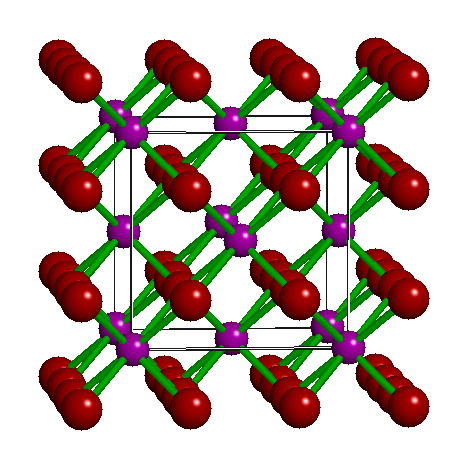
\includegraphics[width=\linewidth]{UO2/UO2.png}
  \caption{Uraninite}
\end{wrapfigure}
The data are the UO$_2$ shown in Shelly's paper on \textit{Reduction
  of Uranium(VI) by Mixed Iron(II)/Iron(III) Hydroxide (Green Rust): 
  Formation of UO$_2$ Nanoparticles}:
\href{http://dx.doi.org/10.1021/es0208409}{\texttt{http://dx.doi.org/10.1021/es0208409}}

The fitting model follows rather closely to what is described in that
paper, particularly the content of Table 2, although I allow S$_0^2$
to float (\texttt{amp}).  Along with an energy shift (\texttt{enot}),
a $\Delta R$ and $\sigma^2$ for the first shell O (\texttt{dro} and
\texttt{sso}), a $\Delta R$ and $\sigma^2$ for the second shell U
(\texttt{dru} and \texttt{ssu}), and a $\Delta R$ and $\sigma^2$ for
the third shell O (\texttt{dro2} and \texttt{sso2}), there is a
parameter for the number of U scatterers (\texttt{nu}).

The model includes the same 6 paths given in Table 2 of Shelly's
paper.

\texttt{amp} is unitless.  \texttt{enot} is eV.
\texttt{dro}, \texttt{dru}, and \texttt{dro2} are \AA.
\texttt{sso}, \texttt{ssu}, and \texttt{sso2} are \AA$^2$.


\def\feffmaterial{UO2}
\def\feffrone{3}
\def\feffrtwo{4}
\def\feffrthree{5}
\def\feffrfour{5.5}
\def\feffrfive{6}
\def\fefffirst{}

\scriptsize
\input{\feffmaterial/\feffmaterial}
\fitplots


\section{UO$_2$, first shell}

\normalsize
This fit includes only the first shell, and a standard 4-paramater
model.  \texttt{amp} is unitless.  \texttt{enot} is eV, \texttt{dro}
is \AA, and \texttt{sso} is \AA$^2$.

\def\fefffirst{_1st}

\small
\input{\feffmaterial/\feffmaterial\fefffirst}
\fitplots


%%%%%%%%%%%%%%%%%%%%%%%%%%%%%%%%%%%%%%%%%%%%%%%%%%%%%%%%%%%%%%%%%%%%%%
%%%%%%%%%%%%%%%%%%%%%%%%%%%%%%%%%%%%%%%%%%%%%%%%%%%%%%%%%%%%%%%%%%%%%%
%%%%%%%%%%%%%%%%%%%%%%%%%%%%%%%%%%%%%%%%%%%%%%%%%%%%%%%%%%%%%%%%%%%%%%



\section{BaZrO$_3$}
\normalsize


\begin{wrapfigure}{r}{0.25\textwidth}
  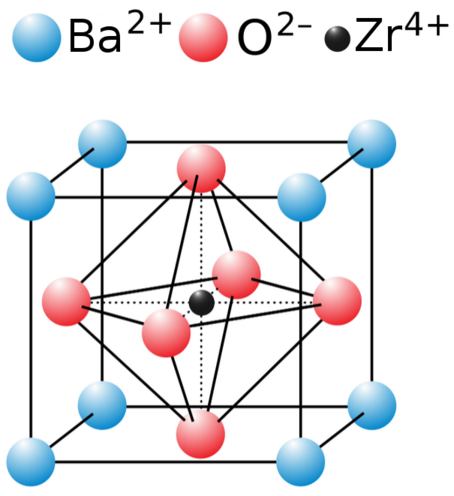
\includegraphics[width=\linewidth]{BaZrO3/perovskite.png}
  \caption{The perovskite structure.}
\end{wrapfigure}
In this paper on the Zr edge of BaZrO$_3$
\href{http://dx.doi.org/10.1016/0921-4526(94)00654-E}
{\texttt{http://dx.doi.org/10.1016/0921-4526(94)00654-E}}, Haskel et
al. (and what a sordid ``et al.'' \textit{that} was) proposed that
shortcomings of \textsc{feff}'s potential model could be accommodated
by floating an energy shift parameter for each scatterer species.  The
concept is that doing so approximates the effect if errors in the
scattering phase shifts.

The data are the same as in that paper, although the fitting model is
slightly different.  Rather than floating $\Delta R$ parameters for
each shell, I used a volumetric expansion coefficient
(\texttt{alpha}).  Along with S$_0^2$ (\texttt{amp}), there are energy
shofts for each scatterer (\texttt{enot}, \texttt{ezr}, and
\texttt{eba}) and $\sigma^2$ parameters for each scatterer
(\texttt{sso}, \texttt{sszr}, and \texttt{ssba}.  The fourth shell O
is included in the fit.  It gets a $\sigma^2$ (\texttt{sso2})but uses
the energy shift for the O scatterer.

BaZrO$_3$ is a true perovskite.  Zr sites in the octahedral B site.  A
variety of collinear multiple scattering paths at the distance of the
third shell Zr scatterer are included in the fit.  The energy shifts
are parameterized as described in the paper.

\texttt{amp} and \texttt{alpha} are unitless.  \texttt{enot},
\texttt{ezr}, and \texttt{eba} are eV.  \texttt{sso}, \texttt{sszr},
\texttt{ssba}, and \texttt{sso2} are \AA$^2$.


\def\feffmaterial{BaZrO3}
\def\feffrone{3}
\def\feffrtwo{4}
\def\feffrthree{5}
\def\feffrfour{5.5}
\def\feffrfive{6}
\def\fefffirst{}

\scriptsize
\input{\feffmaterial/\feffmaterial}
\fitplots


\section{BaZrO$_3$, first shell}
\normalsize
This fit includes only the first shell, and a standard 4-paramater
model.  \texttt{amp} is unitless.  \texttt{enot} is eV, \texttt{delr}
is \AA, and \texttt{sso} is \AA$^2$.

\def\fefffirst{_1st}

\small
\input{\feffmaterial/\feffmaterial\fefffirst}
\fitplots

%%%%%%%%%%%%%%%%%%%%%%%%%%%%%%%%%%%%%%%%%%%%%%%%%%%%%%%%%%%%%%%%%%%%%%
%%%%%%%%%%%%%%%%%%%%%%%%%%%%%%%%%%%%%%%%%%%%%%%%%%%%%%%%%%%%%%%%%%%%%%
%%%%%%%%%%%%%%%%%%%%%%%%%%%%%%%%%%%%%%%%%%%%%%%%%%%%%%%%%%%%%%%%%%%%%%

% \newpage

% \section{methyltin}
% \normalsize

% \small
% \input{methyltin/methyltin}

% \newpage

%%%%%%%%%%%%%%%%%%%%%%%%%%%%%%%%%%%%%%%%%%%%%%%%%%%%%%%%%%%%%%%%%%%%%%
%%%%%%%%%%%%%%%%%%%%%%%%%%%%%%%%%%%%%%%%%%%%%%%%%%%%%%%%%%%%%%%%%%%%%%
%%%%%%%%%%%%%%%%%%%%%%%%%%%%%%%%%%%%%%%%%%%%%%%%%%%%%%%%%%%%%%%%%%%%%%



\section{bromoadamantane}
\normalsize


\begin{wrapfigure}{r}{0.25\textwidth}
  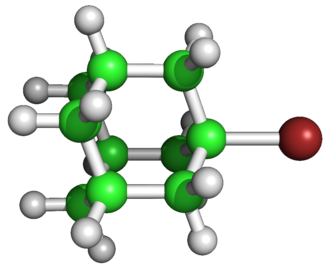
\includegraphics[width=\linewidth]{bromoadamantane/bromoadamantane.png}
  \caption{~\hfill\break 1-bromoadamantane}
\end{wrapfigure}

The data are 1-bromoadamantane.  Adamantane is a cycloalkane, meaning
that it is a hydrocarbon with rings of carbon atoms.  It is also a
diamondoid, meaning that it is a strong, stiff, 3D network of covalent
bonds.  1-bromoadamantane has one hydrogen atom replaced by a bromine
atom.

The material was supplied by my colleague Alessandra Leri of Manhattan
Marymount College in the form of a white powder.  This powder was
spread onto kapton tape which was folded to make a sample with an edge
step of about 1.7.

This is an interesting test case because it is a molecule (thus the
entire molecule can be included in the self-consistency calculation)
and because there is measureable scattering from the neighboring
hydrogen atoms.  While the $\sigma^2$ of the hydrogen scatterers is not
well-determined, the fit is statistically significantly worse when the
hydrogen scatterers are excluded.

The fit includes the nearest neighbor C, the next three C atoms, and
the neighboring 6 hydrogen atoms.  The DS triangle paths involving the
first and second neighbor C atoms are also included.  The fitting
model assumes that the adamanatane anion is very rigid compared to the
Br-C bond.  Thus, the formula explained in 
\href{http://dx.doi.org/10.1088/1742-6596/190/1/012026}%
{\texttt{http://dx.doi.org/10.1088/1742-6596/190/1/012026}} is used to
constrain the second neighbor C distance to the first neighbor C
$\Delta R$ parameter.



\def\feffmaterial{bromoadamantane}
\def\feffrone{8}
\def\fefffirst{}

\small
\input{\feffmaterial/\feffmaterial}
\fitthreeplots


\section{bromoadamantane, first shell}
\normalsize

This fit includes only the first shell, and a standard 4-paramater
model.  \texttt{amp} is unitless.  \texttt{enot} is eV, \texttt{delr}
is \AA, and \texttt{ss} is \AA$^2$.

\def\fefffirst{_1st}

\small
\input{\feffmaterial/\feffmaterial\fefffirst}
\fitthreeplots




%%%%%%%%%%%%%%%%%%%%%%%%%%%%%%%%%%%%%%%%%%%%%%%%%%%%%%%%%%%%%%%%%%%%%%
%%%%%%%%%%%%%%%%%%%%%%%%%%%%%%%%%%%%%%%%%%%%%%%%%%%%%%%%%%%%%%%%%%%%%%
%%%%%%%%%%%%%%%%%%%%%%%%%%%%%%%%%%%%%%%%%%%%%%%%%%%%%%%%%%%%%%%%%%%%%%



\section{uranyl hydrate}
\normalsize

\begin{wrapfigure}{r}{0.25\textwidth}
  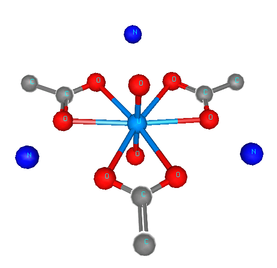
\includegraphics[width=\linewidth]{uranyl/uranyl.png}
  \caption{The uranyl motif from sodium uranyl triacetate.}
\end{wrapfigure}

The data are the uranyl hydrate shown in Shelly's paper on
\textit{X-ray absorption fine structure determination of pH-dependent
  U-bacterial cell wall interactions},
\href{http://dx.doi.org/10.1016/S0016-7037(02)00947-X}
{\texttt{http://dx.doi.org/10.1016/S0016-7037(02)00947-X}}

This is an interesting test case because it involves very short
($\sim1.78$\,\AA) uranium-oxygen bonds.  The \texttt{AFOLP} card was
used to run \textsc{feff}6.  The \texttt{FOLP} card with a value of
0.9 for each potential was used to get \textsc{feff}8.5 to run to
completion.

Following the lead of that paper, \textsc{feff} was run on the crystal
sodium uranyl triacetate.  The relevant bit of the structure is shown
in the figure.  For the fitting model, scattering paths related to the
axial and equatorial O atoms (red balls) are used in the fit.  Other
paths are unused.  The parameterization given in Tables 2 and 5 is
used in this fit.

There is an S$_0^2$ (\texttt{amp}) and an energy shift
(\texttt{enot}).  The axial and equatorial oxyegn atoms each get a
$\Delta R$ (\texttt{deloax} and \texttt{deloeq}) and a $\sigma^2$
(\texttt{sigoax} and \texttt{sigoeq}).

\texttt{amp} is unitless.  \texttt{enot} is eV.
\texttt{deloax} and \texttt{deloeq} are \AA.
\texttt{sigoax} and \texttt{sigoeq} are \AA$^2$.

\def\feffmaterial{uranyl}
\def\feffrone{2.5}
\def\feffrtwo{2.9}
\def\feffrthree{4.0}
\def\feffrfour{5.2}
\def\feffrfive{6.8}
\def\fefffirst{}

\small
\input{\feffmaterial/\feffmaterial}
\fitplots


\end{document}

%%% Local Variables:
%%% mode: latex
%%% TeX-master: t
%%% TeX-parse-self: t
%%% TeX-auto-save: t
%%% TeX-auto-untabify: t
%%% TeX-PDF-mode: t
%%% End:
